
\documentclass[a4paper,12pt]{article}

\usepackage[russian]{babel}
\usepackage[utf8]{inputenc}
\usepackage{amsmath}
\usepackage{amssymb}
\usepackage{appendix}
\usepackage{cmap}
\usepackage{color}
\usepackage{enumerate}
\usepackage{fancyhdr}
\usepackage{framed}
\usepackage{graphicx}
\usepackage{indentfirst}
\usepackage{longtable}
\usepackage{amsfonts}
\usepackage{multirow}
\usepackage{sectsty}
\usepackage{totcount}
\usepackage{url}
\usepackage{xspace}
\usepackage{svg}

\definecolor{darkblue}{rgb}{0,0,.5}
\usepackage[colorlinks, linkcolor=black, menucolor=black, citecolor=black, urlcolor=darkblue]{hyperref}


\newcommand{\EN}[1]{{#1}}
\newcommand{\CODE}[1]{{\ttfamily #1}}
\newcommand{\setof}[1]{\ensuremath{\left \{ #1 \right \}}}
\newcommand{\tuple}[1]{\ensuremath{\left \langle #1 \right \rangle }}

\fancyhf{}
\fancyfoot[C]{\normalsize \thepage}
\renewcommand{\headrulewidth}{0pt}
\renewcommand{\footrulewidth}{0pt}

%%Modifying captions for figures and tables:
\makeatletter
\long\def\@makecaption#1#2{%
\vspace{\abovecaptionskip}%
\sbox{\@tempboxa}{\large #1.~#2}
\ifdim \wd\@tempboxa >\hsize
{\large #1.~#2}\par
\else
\global\@minipagefalse
\hbox to \hsize {\hfill {\large #1.~#2}\hfill}%
\fi
\vspace{\belowcaptionskip}}

\renewcommand{\baselinestretch}{1.2}
%%\sectionfont{\LARGE}
\sectionfont{\Large}
\subsectionfont{\Large}
\subsubsectionfont{\Large}
\setlength{\belowcaptionskip}{6pt}
\makeatletter \renewcommand{\@biblabel}[1]{#1.\hfill}

\makeatletter 
\def\redeflsection{\def\l@section{\@dottedtocline{1}{1.5em}{7.8em}}} 
\renewcommand\appendix{\par 
\setcounter{section}{0}% 
\setcounter{subsection}{0}% 
\def\@chapapp{\appendixname}% 
\addtocontents{toc}{\protect\redeflsection} 
\def\thesection{\appendixname\hspace{0.2cm}\@Asbuk\c@section}} 
\makeatother 

\textwidth = 17cm
\oddsidemargin= 0 pt
\topmargin = -1cm
\headheight = 0cm
\headsep = 0cm
\textheight = 26.5cm

\newtotcounter[auxfile=totals.aux]{figurecnt}
\def\oldfigure{} \let\oldfigure=\figure
\def\figure{\stepcounter{figurecnt}\oldfigure}
\newtotcounter[auxfile=totals.aux]{bibcnt}
\def\oldbibitem{} \let\oldbibitem=\bibitem
\def\bibitem{\stepcounter{bibcnt}\oldbibitem}
\regtotcounter[auxfile=totals.aux]{page}


\begin{document}
\sloppy
\large
\thispagestyle{empty}
\begin{center}
МИНОБРНАУКИ РОССИИ\\
ТОМСКИЙ ГОСУДАРСТВЕННЫЙ УНИВЕРСИТЕТ\\
Факультет информатики\\
Кафедра теоретических основ информатики\\
\end{center}

УДК 681.03

\vspace{0.5cm}

\begin{flushright}
ДОПУСТИТЬ К ЗАЩИТЕ В ГАК\\
Зав.кафедрой, доцент, к.т.н.\\
\makebox[3cm]{\hrulefill}А.Л.Фукс\\
«\makebox[0.8cm]{\hrulefill}»\makebox[1.5cm]{\hrulefill}2013 г.\\
\end{flushright}



\begin{center}

\vspace{1.5cm}
{\bf БАКАЛАВРСКАЯ РАБОТА}\\
\vspace{0.5cm}
АНАЛИЗ ТОНАЛЬНОСТИ СООБЩЕНИЙ СОЦИАЛЬНОЙ СЕТИ TWITTER

\vspace{0.5cm}
по основной образовательной программе подготовки бакалавров\\
010400 --- Информационные технологии

\vspace{0.5cm}

Цветков Алексей Дмитриевич


\end{center}

\vskip 0pt plus 1filll

\begin{tabbing}
\hspace{10cm}\=Руководитель ВКР\\
\>\makebox[3cm]{\hrulefill}М.С.Пожидаев\\
\>«\makebox[0.8cm]{\hrulefill}»\makebox[1.5cm]{\hrulefill}2013 г.\\
\end{tabbing}

\begin{tabbing}
\hspace{10cm}\=Автор работы\\
\>Студент группы №1491\\
\>\makebox[3cm]{\hrulefill}А.Д.Цветков\\
\end{tabbing}

\vspace*{1cm}

\begin{center}
Томск 2013
\end{center}
\normalsize

\newpage
\begin{center}
	\textbf{Реферат}
\end{center}

Выпускная квалификационная работа \total{page}~с., \total{figurecnt}~рис., источников \total{bibcnt}, табл. 3.

АНАЛИЗ ТОНАЛЬНОСТИ, МАШИННОЕ ОБУЧЕНИЕ, СОЦИАЛЬНЫЕ СЕТИ, TWITTER, PYTHON, DJANGO

%TODO
\newpage
\pagestyle{fancy}
\renewcommand{\contentsname}{Оглавление}
\tableofcontents 
\newpage
\section*{Введение}
\addcontentsline{toc}{section}{\hspace{7mm}Введение}

``Анализ тональности'' (\textit{Sentiment Analysis}) ---  класс методов анализа 
содержимого, предназначенный для автоматизированного выявления в текстах 
эмоционально окрашенной лексики и эмоциональной оценки авторов по 
отношению  к объектам, речь о которых идёт в тексте~\cite{wikisent}. 

Мнения других людей влияли на наш процесс принятия решений ещё до 
распространения интернета. Однако, если раньше было возможным узнать мнение 
лишь у ограниченного числа знакомых, то в последнее десятилетие, в связи с 
ростом популярности сети интернет, всё большее значение приобретают отзывы, 
оставляемые пользователями в интернет-магазинах, блогах, социальных сетях, а 
также специализированных ресурсах (``Яндекс.Маркет'', ``Кинопоиск''). 

Согласно опросу, проведённому компанией Dimensional Research~\cite{dimresearch}, 
88\% опрошенных считают, что чтение положительных или отрицательных 
отзывов в интернете влияет на их решение при покупке товаров (что согласуется с 
данными, полученными при проведении аналогичного опроса в АиФ России~\cite{aif}). 
Отзывы на качество обслуживания также непосредственно влияют на продажи: 
продажи интернет-магазинов с рейтингом ``5 звёзд'' на ``Яндекс.Маркете'' на 55\% 
больше магазинов с рейтингом ``4 звезды''~\cite{medianation}.

Всё чаще пользователи оставляют отзывы не на специализированных 
сайтах отзывов, а в социальных сетях. 
Отзывы в социальных сетях оставляет на 10\% большее число покупателей, чем на 
специализированных сайтах-агрегаторах~\cite{dimresearch}.
Так как социальные сети содержат не только отзывы, а объём сообщений слишком 
велик для ручной обработки, актуальной является задача автоматического поиска 
и классификации отзывов.
 
``Твиттер'' (\textit{Twitter}) --- одна из самых популярных социальных сетей. 
Число активных пользователей превышает 200 миллионов, и они оставляют более 
400 миллионов сообщений в день~\cite{twitter_users}. 
Ограничение на длину сообщения (140 символов), большой набор используемой 
лексики, сленга и грамматических ошибок делают автоматический поиск и анализ
мнений нетривиальной задачей.

Методы машинного обучения применяются в задачах определения тональности 
уже долгое время~\cite{panglee}, однако их применение в сегменте микроблогов 
началось сравнительно недавно~\cite{distsuperv}.

\vspace{0.5cm}

Целью данной работы является исследование методов автоматического 
определения тональности на основе методов машинного обучения в социальной 
сети Twitter. 

Для достижения поставленной цели требуется:

\begin{enumerate}

\item 
Дать обзор существующим исследованиям в области анализа тональности.

\item 
Изучить и реализовать основные алгоритмы машинного обучения, используемые 
для решения задачи автоматического определения тональности.

\item 
Исследовать качество работы алгоритмов, выявить их достоинства и недостатки.

\item 
Создать веб-приложение для практического использования автоматического 
определения тональности в социальной сети Twitter. 

\end{enumerate}
\newpage
\section{Обзор предметной области}

\subsection{Терминология}

 В рамках данной работы используются терминология предметной области, которую необходимо пояснить.

``{\bfАнализ тональности}'' (\textit{sentiment analysis}), ``{\bfанализ мнений}''(\textit{opinion mining}) --- названия предметной области.

{\bfОбъектом} анализа тональности может являться любая сущность, относительно которой выражается мнение. Например, это может быть продукт, сервис, организация или событие. Объект может обладать множеством \textit{компонентов} (составных частей) и \textit{атрибутов} (свойств), вместе составляющих множество {\bfаспектов} (\textit{features})~\cite{multi_faceted}.

Конкретная модель телефона --- объект. Он состоит из компонентов (\textit{экран, аккумулятор, камера}) и обладает набором атрибутов (\textit{качество передачи голоса, размер}), которые вместе составляют множество аспектов. Мнение может быть выражено, как о самом объекте, так и о любом из его аспектов.

В сообщении ``Мне так нравится новый iPhone. Качество экрана просто потрясающее!'' первое предложение выражает положительное мнение о самом объекте ``iPhone'', а второе --- о его аспекте ``экран''.

{\bfАвтор мнения} (\textit{opinion holder}) --- человек или организация, которые выражают это мнение. 

{\bfТональность мнения} (\textit{opinion orientation}) --- эмоциональная оценка, даваемая автором мнения объекту и/или любому из его аспектов, например \textit{положительная} или \textit{отрицательная} . Строго говоря, тональность может принимать большее число значений, однако чаще всего используются именно эти классы. Часто в литературе можно встретить использование значения \textit{нейтральной} тональности, однако его интерпретация неоднозначна. 
В некоторых работах~\cite{panglee} нейтральная тональность определяется, как промежуточное значение между положительной и отрицательной, а в некоторых, как отсутствие субъективной оценки. В данной работе автор работы придерживается последней интерпретации из-за трудности формализации промежуточного значения. Например, в высказывании ``посредственный экран'' оценка, даваемая автором мнения аспекту ``экран'', является скорее негативной, несмотря на то, что слово ``посредственный'' определяется в словаре, как ``заурядный, средний''~\cite{wiki_middling}.

{\bfМоделью объекта} $o$ называется конечное множество аспектов $F = \setof{f_1, f_2, \ldots , f_n}$, которое включает в себя сам объект в качестве особого аспекта.

{\bfМнения} делятся на два типа~\cite{multi_faceted}:
\begin{enumerate}

\item{
  {\bfПростое} мнение (\textit{direct opinion}). Простое мнение формально определяется, как кортеж \tuple{A, o, f, oo, t, d}, где в документе $d$ автором мнения $A$ аспекту $f$ объекта $o$ дана оценка $oo$ в момент времени $t$. Например, в высказывании ``В Ubuntu очень красивый интерфейс'' автор мнения дал положительную оценку ``красивый'' аспекту ``интерфейс'' объекта ``Ubuntu''.
}

\item{
  {\bfСравнительное} мнение(\textit{comparative opinion}). Сравнительное мнение характеризуется тем, что автор $A$ предпочёл одному или нескольким объектам из множества $O_1$ один или несколько объектов из множества $O_2$, давая сравнительную оценку $oo$ их аспекту $f$. Например, в высказывании ``Интерфейс Ubuntu проще Windows 8'' автор мнения предпочёл объект ``Ubuntu'' объекту ``Windows 8'', дав аспекту ``интерфейс'' сравнительную оценку ``проще''. 
}

\end{enumerate}

В работе также используется терминология, специфичная для Twitter.

{\bfМикроблог} (\textit{microblog}) --- аналог обычного веб-блога (интернет-дневника), с ограничением на длину сообщения (в Твиттере она составляет 140 символов). 

{\bfТвит} (\textit{tweet}) --- сообщение пользователя в Твиттере. Может включать в себя текст, упоминание другого пользователя, гиперссылки и хештэги.

{\bfРетвит} (\textit{retweet}) --- возможность скопировать сообщение другого пользователя в свою ленту (с сохранением авторства). Существует, две разновидности --- нативный (предоставляемый платформой) и текстовый (сообщение, начинающееся с ``RT @имя\_автора:'').

{\bfХештэг} (\textit{hashtag}) --- это слово или фраза, которым предшествует символ \#. Пользователи могут объединять группу сообщений по теме или типу с использованием хэштегов — слов или фраз, начинающихся с \#. В Twitter в хештэгах можно использовать латинские и кириллические буквы, цифры и знаки подчёркивания, однако часто пользователи не используют знаки подчёркивания (``\#отличныйдень''вместо ``\#отличный\_день'').

{\bfУпоминание} (\textit{mention}) --- ссылка на другого пользователя.  Начинается с символа @, после чего идёт никнейм другого пользователя, состоящий из символов латинского алфавита, цифр и знаков подчёркивания. Пользователям приходят уведомления, когда их кто-то упомянул. Иногда используется вместо хештэгов для группировки сообщений по темам (например, вместо ``\#microsoft'' используется ``@microsoft'').
\subsection{Задачи анализа тональности}

Основные задачи, решаемые в области анализа тональности, 
включают в себя~\cite{panglee}:
\begin{enumerate}


\item {
  Задача определения документов или частей документа, которые содержат в себе 
  мнение (\textit{subjectivity detection}). Для документов эта задача сводится к 
  задаче бинарной текстовой классификации на классы {\bfсубъективных} (
  содержащих мнение) и {\bfобъективных} (содержащих факты) документов.
}

\item {
  Задача определения тональности. Чаще всего встречается определение 
  тональности на уровне документа (\textit{document-level sentiment classification}). 
  Формально задача определяется так: 
  из множества $D$ документов, содержащих мнения, для каждого $d \in D$, 
  который содержит высказывание об объекте $o$, необходимо определить 
  тональность $oo$ аспекта $f$~\cite{sentsubj}. 
  Также, определение тональности может быть осуществлено на уровне 
  предложения (\textit{sentence-level sentiment classification}) или аспекта (\textit{
  feature-level sentiment classification}).

  Существующие решения делают следующиее допущение: документ $d$, 
  содержащий мнение, выражает мнение об одном объекте $o$, 
  от одного автора $A$. В общем случае автор документа может выражать мнение 
  относительно нескольких объектов, однако в случае отзывов (и особенно в 
  контексте Twitter) в большинстве случаев это допущение справедливо для 
  простых (не сравнительных) мнений.

  Учитывая допущение, эта задача сводится к бинарной текстовой классификации 
  на классы {\bfположительных} (позитивных) и {\bfотрицательных} (негативных) 
  документов.
}

\item {
  Наконец, необходимо представить информацию о мнениях в некоторой краткой 
  сводке. Это может быть:
  
  \begin{itemize}

  \item Агрегация пользовательских оценок.
  \item Идентификация групп авторов, имеющих схожие мнения.
  \item Выявление пунктов согласия и противоречия.
  \item Статистическое или текстовое обобщение документов.

  \end{itemize}
}

\end{enumerate}

Задачи 1 и 2 можно рассматривать, как задачи текстовой классификации. Решение 
этих задач можно получить с помощью иерархической бинарной классификации (
сначала документ классифицируется, как объективный или субъективный, затем 
субъективные документы --- как положительные или отрицательные) или с 
помощью классификации документа по трём классам \{положительный, 
нейтральный, отрицательный\}. 

Задача определения тональности встречается чаще всего, поэтому далее в работе 
будет подразумеваться именно она.
\subsection{Проблемы автоматического определения тональности}

Проблемы, возникающие при автоматическом определении тональности, можно 
разделить на общие и специфичные для микроблогов.

\vspace{0.5cm}

Среди общих проблем можно выделить следующие:

\begin{enumerate}

\item 
Зависимость значения тональности от предметной области. Так, в области 
фильмов слово ``непредсказуемый'' может иметь положительный оттенок, 
однако в области клиентского обслуживания это не так.
При использовании методов обучения с учителем, алгоритм классификации (
например, наивный Байесовский классификатор) сам формирует значения 
тональности из обучающей выборки, поэтому для правильной классификации 
достаточно, чтобы обучающая и тестовые выборки имели общую предметную 
область.

На практике запросы пользователей не обязательно ограничены
какой-либо одной областью, поэтому возможна категоризацая текста в два 
прохода: сначала осуществляется тематическая классификация 
документа, затем классификация тональности.

\item 
Использование отрицания может изменить тональность остальной части 
высказывания на обратную. 
Например, в высказывании ``Раньше мне \textit{очень нравились} смартфоны Nokia. Качество сборки в Lumia 800, действительно, \textit{на высоте}. \textit{Однако}, Windows Phone 7 \textit{всё портит}''. 
В первом и втором предложении автор высказывает положительное мнение, но 
из-за использования отрицания в третьем предложении общая тональность 
относительно объекта ``Nokia'' отрицательная. 

Для методов машинного обучения, использующих модель 
типа ``набор слов'' (\textit{bag-of-words}), 	в качестве простой эвристики можно 
искусственно добавлять частицу ``не'' к соседним словам (к примеру, для 
высказывания ``Мне не очень нравится камера iPhone'' получится строка 
``Мне не не\_очень не\_нравится камера iPhone''), однако это не очень точное моделирование отрицания (кроме того, отрицание может быть выражено неявно).	

Исследования в данной области находятся на очень ранней стадии~\cite{Wiegand2010}.

\item 
Использование сарказма плохо поддаётся автоматическому определению. 
Высказывания, содержащие сарказм могут иметь общую тональность, 
обратную тональности отдельных слов 
(``\textit{Отличная} книга для страдающих бессонницей!''), 
или выражать мнение в скрытой форме (вопрос ``Где я?'' 
в обзоре GPS-навигатора). В этом случае, сарказм может с трудом распознаваться даже людьми. 

В одной из последних работ в данной области авторам удалось 
добиться точности на уровне 78\% на коллекции отзывов на товары, используя 
метод частичного обучения (\textit{semi-supervised learning})~\cite{Tsur2010}.

\item 
Значение тональности зависит от того, кому необходимо провести анализ. 
Так, для компании Samsung высказывание ``У Samsung показывает отличные продажи :)'' несёт положительное значение тональности, а для компании Nokia --- наоборот.

\end{enumerate}

\vspace{0.5cm}

К специфичным для Твиттера проблемам относятся:

\begin{enumerate}

\item 
Большой словарь употребимых слов.  
Как показывают исследования~\cite{Saif2012}	, 93\% встречающихся слов 
употребляются менее, чем 10 раз (78\% на корпусе рецензий фильмов из IMDB). 
Это объясняется частым использованием сленга, намеренным и ненамеренным искажением написания слов, использованием разных регистров при написании одного и того же слова.

\item 
Малое количество слов в каждом сообщении. 
Из-за ограничения на длину сообщения, средняя длина сообщения на 
английском составляет 14 слов или 78 символов~\cite{Go2009}.

\item 
Большие объёмы данных. 
Пользователи публикуют более 400 миллионов сообщений в день, 
1\% сообщений доступны всем желающим, 
50\% сообщений доступны для компаний-партнёров~\cite{streaming}. 
Даже 1\% --- это более 40 миллионов сообщений в день, что является 
достаточно большим объёмом для обработки локально. 
Так как все сообщения можно сначала обработать независимо, 
а затем агрегировать результаты, 	разумным 
может быть применение распределённых вычислений, к примеру, 
использование парадигмы MapReduce~\cite{Lin2012, sentiment_mapreduce}.

\end{enumerate}
\subsection{Методы автоматического определения тональности}

Основные подходы к определению тональности можно 
разделить на следующие категории~\cite{Irokez2012}:
\begin{enumerate}

\item 
Подход, основанный на правилах (\textit{rule-based approach}), 
заключается в применении набора правил, выявленного экпертами на основе 
анализа предметной области. 

Пример такого правила:
\begin{framed}

	Если высказывание содержит один или несколько положительных 
	прилагательных из набора 
	\{``хороший'', ``качественный'', ``свежий'' \ldots \} и 
	не содержит прилагательных из набора 
	\{``бездарный'', ``ужасный'', ``жуткий'' \ldots \}, 
	то значение тональности ``положительное''.

\end{framed}

Достоинства подхода:
\begin{itemize}

	\item 
	Может показывать хорошие результаты при большом наборе правил.

\end{itemize}

Недостатки подхода:
\begin{itemize}
	
	\item   
	Создание большого набора достаточно трудозатрано.  
	
	\item  
	Применение этого подхода для микроблогов может быть проблематично из-за 
	``зашумленности'' данных. 

\end{itemize} 

Более подробно определение тональности с помощью подходов, 
основанных на правилах, описано в~\cite{rule_romip1, rule_romip2}.


\item 
Подход, основанный на использовании словарей оценочной лексики 
(\textit{affective lexicons}). 
Для каждого слова, встречаемого в документе, из словаря получают значение 
тональности. Чтобы получить итоговую тональность необходимо взять среднее 
арифметическое или вычислить сумму значений тональности всех слов из 
документа. 

Достоинства подхода:
\begin{itemize}

	\item 
	Простота использования. 

\end{itemize}

Недостатки подхода:
\begin{itemize}

	\item 
	Не универсальность: для каждой предметной области требуется свой словарь. 

	\item
	Создание такого словаря может быть проблематичным.

\end{itemize} 

Для английского языка в качестве такого словаря можно использовать SentiWordNet~\cite{sentiwordnet} или ANEW~\cite{anew}.

\item 
Подходы, основанные на обучении с учителем (\textit{supervised learning}). 
Обучение с учителем --- один из разделов машинного обучения. Алгоритм 
классификации тренируется на основе обучающей выборке (корпусе), состоящей 
из документов, классы которых заранее известны. 

Достоинства подхода:
\begin{itemize}
	
	\item
	Хорошая точность при определении тональности.

	\item
	На основе обучающей выборки классификатор самостоятельно выделяет 
	признаки, влияющие на тональность. 
	Таким образом, проблема зависимости от предметной области решается 
	с помощью использования обучающей выборки из той же области. 

	\item
	Существует множество способов улучшить точность.

\end{itemize}

Недостатки подхода:
\begin{itemize}

	\item
	Требуется размеченная обучающая выборка.

	\item
	Результаты могут сильно зависеть от выбранного алгоритма, его параметров, 
	обучающей выборки.

\end{itemize} 

\item 
Подходы, основанные на обучении без учителя (\textit{unsupervised learning}). 
Обучение без учителя является ещё одним из разделов машинного обучения. 
Отличие состоит в том, что в этом случае для тренировки алгоритма используется 
обучающая выборка, состоящей из документов, классы которых заранее 
неизвестны (или известны, но эта информация не используется алгоритмом).

Достоинства подхода:
\begin{itemize}

	\item
	Для обучения не требуется размеченная выборка. 

\end{itemize}

Недостатки подхода:
\begin{itemize}

	\item
	Точность обычно значительно ниже, чем у алгоритмов, основанных на обучении с учителем.

\end{itemize} 

\end{enumerate}

Так как подходы, основанные на обучении с учителем, 
показывают хорошие результаты при анализе традиционных 
блогов и сайтов рецензий, далее в работе даётся их подробное описание, 
описываются способы представления данных и улучшения точности  работы 
алгоритмов, а также результаты работы в области микроблогов.

\newpage
\section{Определение тональности с помощью методов машинного обучения} 
\label{sec:sec_mlsent}

\subsection{Задача классификации при обучении с учителем}

В общем виде задача текстовой классификации определяется следующим 
образом~\cite{Manning2008}. 
Пусть существует описание документа $d \in \mathbb{X}$, где $\mathbb{X}$ --- векторное пространство документов, и фиксированный набор классов 
$\mathbb{C} = \setof{c_1, c_2, \ldots, c_m}$. 
Из обучающей выборки (множества документов с заранее известными классами)
$\mathbb{D} = \{\tuple{d, c} \mid \tuple{d, c} \in \mathbb{X} \times \mathbb{C}\}$
с помощью метода обучения $\Gamma$ необходимо получить классифицирующую 
функцию (или классификатор) 
$\Gamma(\mathbb{D}) = \gamma$, которая отображает документы в классы $\gamma: \mathbb{X} \rightarrow \mathbb{C}$.

В задаче определения тональности множество $\mathbb{C}$ состоит 
из двух элементов \{положительный, отрицательный\}.

\subsubsection{Представление данных}
Все документы из обучающей и тестовой выборки представляют собой $n$-мерные признаковые векторы 
(англоязычное название \textit{feature vector}, однако не стоит путать признаки с аспектами). 

В задачах обработки текста на естественном языке популярно представление 
документов в виде $n$-грамм, где $n$-граммы --- последовательности слов длины $n$. 
Для $n = 1$ такая последовательность состоит из одного слова и называется 
юниграммой (модель, которая использует представление в виде юниграмм 
называется ``набор слов'' (\textit{bag-of-words}), так как слова рассматриваются 
независимо друг от друга). Для $n = 2$ такая последовательность называется биграммой, и т.д.

Например, для высказывания ``Сегодня отличный день!'' множество юниграмм 
будет состоять из элементов \{``Сегодня'', ``отличный'', ``день!''\}, а множество
биграмм \{``Сегодня\_отличный'', ``отличный\_день!''\}. 
Стоит отметить, что с ростом $n$, $n$-граммы всё точнее 
отражают оригинальный текст, а потому их ценность
для моделирования произвольного текста падает (в задачах текстовой 
классификации редко используется $n > 3$). Теоретически, использование биграмм
даёт возможность моделировать значение тональности более точно: если 
рассматривать словосочетание ``не нравится'', как набор независимых слов, то
он содержит одно слово с отрицательной тональностью
и одно с положительной, поэтому
классификатор может посчитать, что общая тональность будет близка к нулевой. С 
другой стороны, маловероятно, что биграмма ``не\_нравится'' 
будет использована в положительном контексте.

Таким образом документ определяется как вектор $d = (w_1, w_2, \ldots , w_{|\mathbb{V}|}) $,
где $\mathbb{V}$ --- множество всех уникальных термов из 
обучающей выборки. 

$w_i$ --- вес i-го терма. Популярные способы взвешивания~\cite{wiki_vectorspace}:
\begin{enumerate}

\item 
Булевский вес --- $w_i = 1$ если терм присутствует в документе, иначе 0.

\item
Количество вхождений i-го терма в $d$ 
\begin{equation} 
w_i = n_i
\end{equation}

\item
Частота терма (\textit{TF --- term frequency}) --- отношение числа вхождений i-го терма к общему количеству термов документа.

\begin{equation} 
w_i = tf(t_i, d) = \frac{n_i}{\sum n_k}
\end{equation}

\item
TF-IDF (\textit{IDF --- inverse document frequency}, обратная частота документа) 

\begin{equation} 
idf(t, \mathbb{D} ) = \log \frac{|\mathbb{D}|}{| (d_i \supset t_i) |}
\end{equation}

\begin{equation} 
w_i = tfidf(t_i, d, \mathbb{D} ) = tf(t_i, d) \times idf(t, \mathbb{D} )
\end{equation}

где $|\mathbb{D}|$ --- количество документов в корпусе, $| (d_i \supset t_i) |$ ---
количество документов, в которых встречается $t_i$.

\end{enumerate}


\subsubsection{Определение качества работы классификатора}

Чтобы сравнивать алгоритмы классификации необходимо 
ввести меру оценки качества работы.

Для этого необходима тестовая выборка с заранее известными классами.
По результату работы обученного классификатора на тестовой выборке
для каждого класса считаются следующие значения~\cite{classifier_performance}:
\begin{itemize}
\item $TP$--- количество истинно-положительных результатов.
\item $TN$ --- количество истинно-отрицательных результатов.
\item $FP$ --- количество ложно-положительных результатов.
\item $FN$ --- количество ложно-отрицательных результатов.
\end{itemize}

На основе этих значений считаются меры точности (\textit{precision}) 
и полноты (\textit{recall}):

\begin{equation}
Precision = \frac{TP}{TP+FP}
\end{equation}

\begin{equation}
Recall = \frac{TP}{TP+FN}
\end{equation}

Их смысл в следующем: точность --- доля результатов, которая действительно
принадлежит данному классу, а полнота --- процент найденных результатов
от их общего числа.

Так как при стремлении любой из этих величин к нулю, ценность классификатора 
падает, то для усреднения обоих значений определяется $F_1$-мера, как 
гармоническое среднее точности и полноты:

\begin{equation}
F_1 = \frac{2 (Precision + Recall)}{Precision Recall}
\end{equation}

В отличии от среднего арифметического в случае, если $Precision = 0$, а $Recall = 1$ (или наоборот), среднее будет равняться нулю, а не $\frac{1}{2}$.

Для того, чтобы избежать проблемы переобучения (\textit{overfitting}),
когда модель слишком хорошо работает на примерах, но плохо на реальных данных,
для проверки модели используется метод перекрёстной проверки (\textit{cross-validation}). 
Вся обучающая выборка делится на $k$-частей, затем $\forall i \in \{1, 2, \ldots , k\}$
алгоритм классификации обучается на на всей обучающей выборке, кроме части i,
а тестируется на $i$-й части. Результатом работы считается среднее 
арифметическое по всем проходам. Часто значение $k$ принимают равным 5 или 10.
\subsection{Алгоритмы классификации}

\subsubsection{Наивный Байесовский классификатор}
Наивный Байесовский классификатор основан на теореме Байеса~\cite{naive_bayes}:
\begin{equation}
P(c | d) = \frac{P(d | c) P(c)}{P(d)}
\end{equation}

где
\begin{itemize}

\item
$P(c | d)$ --- апостериорная вероятность того, что документ $d$ принадлежит классу $c$.

\item
$P(d | c)$ --- правдоподобие, вероятность встретить документ $d$ среди всех документов класса $c$.

\item
$P(c)$ --- априорная вероятность класса $c$. 

\item
$P(d)$ --- априорная вероятность документа $d$. 

\end{itemize}

В качестве результирующего выбирается класс с максимальной апостериорной вероятностью:
\begin{equation}
c = \arg\!\underset{c \in \mathbb{C}}{\max} P(c | d)
\end{equation}

Так как плотности распределения чаще всего неизвестны, производится их оценка
по обучающей выборке. При этом оценка вероятности документа в обучающей 
выборке $P(d) = const$, а следовательно не влияет на классификацию.
\begin{equation}
c = \arg\!\underset{c \in \mathbb{C}}{\max} P(d | c) P(c)
\end{equation}

Наивный Байесовский классификатор основан на дополнительном предположении
о том, что классифицирующие признаки являются независимыми, поэтому
условная вероятность документа $P(d | c) \approx P(w_1 | c) P(w_2 | c) \ldots P(w_{|\mathbb{V}|} | c) $, где $w_i \in d$.
\begin{equation}
P(c | d) \approx P(c) \prod\nolimits_{i=1}^{|\mathbb{V}|} P(w_i | c) 
\end{equation}

Для того, чтобы избежать переполнения снизу, обычно произведение
логарифмируется (это изменяет численные значения вероятностных оценок, 
однако значение, при котором достигается максимум, сохраняется).

\begin{equation}
P(c | d) \propto \log P(c) + \sum\nolimits_{i=1}^{|\mathbb{V}|} \log P(w_i | c) 
\end{equation}

Вероятностные оценки определяются следующим образом:

\begin{equation}
P(c) = \frac{\mathbb{D}_c}{|\mathbb{D}|}
\end{equation}

\begin{equation}
P(w_i | c) = \frac{W_{ic}}{\sum\nolimits_{j=1}^{|\mathbb{V}|} W_{jc}}
\end{equation}

где 
\begin{itemize}

\item
$W_{ic}$ --- количество раз сколько i-й терм встречается в документах класса c.

\item
$\mathbb{D}_c$ --- количество документов $d \in \mathbb{D}$ класса c.

\end{itemize}

Достоинства наивного Байесовского классификатора:
\begin{itemize}

\item
Простота реализации.

\item
Быстрый процесс обучения. Вычислительная трудоёмкость обучения $O(|\mathbb{D}| |\mathbb{V}|)$.

\item
Несмотря на то, что предположение о независимости классификационных 
признаков не является верным в естественном языке (значение слова зависят от контекста), 
НБК часто показывает хорошие результаты при текстовой классификации~\cite{thumbs_up}. 

\end{itemize}

Недостатки:
\begin{itemize}

\item
Значения, возвращаемые при классификации, нельзя трактовать, 
как вероятности. Таким образом нельзя ответить на вопрос, 
с какой долей уверенности получился результирующий класс. 

\item
Так как в естественном языке слова не являются независимыми,
НБК не является оптимальным.

\end{itemize}

\subsubsection{Классификация методом максимальной энтропии}

Для каждого признака $w_i$ и каждого класса $c_i \in \mathbb{C}$
определим функцию

\begin{equation}
F_{i, c_i}(d, c) = \left\{
\begin{array}{c l}
    1 & {w_i > 0 \wedge c = c_i}  \\   
    0 & {w_i \leq 0\vee c \neq  c_i}
\end{array}\right.
\end{equation}

Оценка вероятности $P(c | d)$ определяется следующим образом:
\begin{equation}
P(c | d, \lambda) = \frac{1}{Z(d)} \exp{\sum\limits_{i'} \lambda_{i'} F_{i', c}}
\end{equation}

где $Z(d)$ --- функция нормировки:

\begin{equation}
Z(d) = \sum\limits_{c' \in \mathbb{C}} \exp{\sum\limits_{i'} \lambda_{i'} F_{i', c'}}
\end{equation}

$\lambda_{i'}$ --- вес i-го признака. Так как, в отличии от наивного Байеса,
метод максимальной энтропии не делает никаких предположений
об условной независимости признаков, то $\lambda_{i'}$ необходимо
восстанавливать из обучающей выборки.

Это можно сделать, максимизировав функцию логарифмического правдоподобия:
\begin{equation}
L(\mathbb{D}, \lambda) = \sum\limits_{\tuple{d, c} \in \mathbb{D}} \log P(c|d, \lambda)
\end{equation}

Так как все значения $P(c|d, \lambda)$ нормированы по единице, а логарифм является выпуклой функцией, то для максимизации можно воспользоваться
методом градиентного подъёма.

Достоинства метода:
\begin{itemize}

\item
Из-за отсутствия предположений об условной независимости признаков
теоретически может показывать лучшую производительность, чем
НБК.

\end{itemize}

Недостатки метода:
\begin{itemize}

\item
Сложная реализация. Необходимо реализовать градиентный подъём,
определить критерий сходимости, параметр шага.

\item
Обучение медленнее, чем в случае НБК.

\end{itemize}
\subsection{Оценка качества работы алгоритмов}

Оценка алгоритмов в задаче определения тональности проводилась на основе 
тестирования на двух англоязычных размеченных корпусах: Sanders~\cite{Sanders} и SemEval-2013~\cite{SemEval2013},
из которых были удалены нейтральные твиты. Первый корпус содержит 
сообщения из области брендов, второй --- из смешанных областей.


\begin{table}[h]
\caption{Числовые характеристики корпусов.}

	\begin{center}
	    \begin{tabular}{ | l | l | l | l | l | l |}
	    \hline
	    Корпус & Полож. & Отриц. & Всего & Юниграммы & Биграммы \\ \hline
	    Sanders & 502 & 547 & 1049 & 5425 & 12119 \\ \hline
	    SemEval & 3742 & 1565 & 5307 & 25538 & 70775\\ \hline
	    \hline
	    \end{tabular}
	\end{center}
\end{table}


\subsubsection{Нормализация данных}
Перед проверкой алгоритмов необходимо нормализовать данные
для уменьшение размерности и уменьшения ``зашумленности'' данных. 

В качестве способов нормализации использовались:
\begin{enumerate}

\item
Приведение всех букв к нижнему регистру.

\item
Замена всех гиперссылок на токен ``URL''.

\item
Замена всех упоминаний пользователей на токен ``MENTION''.

\item
Замена всех смайликов на токен ``POSITIVE\_SMILEY'' или ``NEGATIVE\_SMILEY'' в 
зависимости от тональности. Замена производилась с помощью регулярных
выражений, список смайликов взят из Википедии~\cite{emoticons}.

\item
Удаление всех хештэгов.

\item
Так как в современном английском не употребляются слова, в которых подряд
идут три и более одинаковых символов, то все такие вхождения заменялись на два символа (``gooood'' и ``goood'' заменяются на ``good'').

\item
Удаление символов пунктуации и замена непечатных символов (табуляции, перевода строки) на пробел.

\end{enumerate}

\begin{table}[h]
\caption{Количество n-грамм после нормализации.}

	\begin{center}
	    \begin{tabular}{ | l | l | l | }
	    \hline
	    Корпус & $n = 1$ & $n = 2$ \\ \hline
	    Sanders &  2871 & 9842 \\ \hline
	    SemEval & 12241 & 58486\\ \hline
	    \hline
	    \end{tabular}
	\end{center}
\end{table}

\subsubsection{Тестирование}

\begin{table}[h]
\caption{Результаты тестирования.}
\newcommand{\mc}[3]{\multicolumn{#1}{#2}{#3}}
	\begin{center}
\begin{tabular}{|c|c|c|c|c|c|c|c|c|c|c|}
\hline 
\mc{3}{|c|}{Классификатор} & \mc{6}{|c|}{Корпус}\\ \hline

Алгоритм & N-грамм & Вес & \mc{3}{|c|}{Sanders} & \mc{3}{|c|}{SemEval}\\ \hline

  &   &   & Precision & \mc{1}{|c|}{Recall} & \mc{1}{|c|}{$F_1$} & \mc{1}{|c|}{Precision} & \mc{1}{|c|}{Recall} & \mc{1}{|c|}{$F_1$}\\ \hline

 NaiveBayes  & 1  & Count & \mc{1}{|c|}{{\bf0.799}} & 0.756 & 0.751 & 0.401 & 0.499 & 0.413\\ \hline

  & 2 & Count & \mc{1}{|c|}{0.709} & 0.698 & 0.695 & \bf{0.768} & 0.545 & 0.508\\ \hline

  &  1+2 & Count & \mc{1}{|c|}{0.795} & {\bf0.765} & {\bf0.762} & 0.719 & 0.509 & 0.436\\ \hline

MaxEnt & 1 & Boolean & \mc{1}{|c|}{0.680} & 0.630  & 0.609 &   &   &  \\ \hline

  & 2 & Boolean  & \mc{1}{|c|}{0.686} &  0.679 & 0.678 &   &   &  \\ \hline

  & 1+2 & Boolean  & \mc{1}{|c|}{0.689} & 0.637  & 0.617  &   &   &  \\ \hline

 Dictionry & & & \mc{1}{|c|}{0.714} & 0.675  & 0.651  & 0.758  & \bf{0.697}  & \bf{0.714} \\ \hline
\end{tabular}
\end{center}

\end{table}

Тестирование проходило с помощью 10-кратной перекрёстной проверки
путём усреднения результатов итераций и затем усреднения результатов по 
классам.

Для сравнения был также использован словарный метод (использовался словарь~\cite{dictionary}, содержащий 6800 слов).

Все алгоритмы были реализованы на языке программирования Python
с применением библиотеки Numpy для быстрых векторных операций.
Для градиентного подъёма в методе максимальной энтропии
были вручную подобраны параметры для приемлемого соотношения
между временем сходимости и качеством работы. 

Из-за времени занимаемого на каждую итерацию (более получаса) метод 
максимальной энтропии не был протестирован на корпусе SemEval. 

На корпусе Sanders наивный Байесовский классификатор показал значительное
превосходство и над словарным методом, и над методом максимальной энтропии.
ММЭ показал результаты на уровне словарного метода, при этом время его работы
занимало существенно большее время. В целом, наилучшие результаты были достигнуты при использовании юниграмм и биграмм в качестве признаков и наивного Байеса в качестве классификатора.

На корпусе SemEval Байесовский классификатор показал немного большую 
точность, однако значение полноты и $F_1$ оказалось на целых 20\% ниже, 
чем у словарного метода. Возможно это связано с тем, что сообщения
в обучающей выборке сильно смещены в сторону положительного класса.
Также стоит заметить, что если первый корпус состоит из сообщений одной области (бренды), 
то второй состоит из сообщений разных областей, поэтому свою роль
могла сыграть зависимость от домена.
\subsection{Улучшение точности работы алгоритмов}

Существует несколько способов улучшить качество работы алгоритмов машинного обучения.

\subsubsection{Выбор признаков}
Выбор признаков (\textit{feature selection}) в первую очередь используется для 
уменьшения размерности признакового пространства. Но так как в данных
присутствует ``шум'' (очень редкие или наоборот очень частые слова, которые
встречаются во всех классах), то уменьшение размерности может улучшить качество и скорость работы алгоритмов. 

Выбор признаков можно осуществлять с помощью следующих способов~cite{wseas2005}:
\begin{enumerate}

\item
На основе частоты встречаемости слова. Самый простой метод: исключаем
из признакового пространства все слова, которые встречались в обучающей
выборке менее $m$ раз. Число $m$ подбирается экспериментально.

\item
На основе взаимной информации (\textit{mutual information})~\cite{mutualinformation}.
Значение взаимной информации показывает взаимосвязь признака
и класса. Для каждого класса берётся $m$ признаков с наибольшими значениями.

Для того, чтобы посчитать значение взаимной информации необходимо рассчитать
следующие значения для каждого слова $word$ и для каждого класса $c$:
\begin{itemize}

\item $N_{1,1}$ --- сколько раз $word$ встречается в документах класса $c$.

\item $N_{0,1}$ --- сколько раз другие слова встречаются в документах класса $c$.

\item $N_{1,0}$ --- сколько раз $word$ встречается в документах других классов.

\item $N_{0,0}$ --- сколько раз другие слова встречаются в документах других классов.

\item $N = N_{1,1} + N_{0,1} + N_{1,0} + N_{0,0}$

\end{itemize}

Тогда значение взаимной информации считается по формуле:

\begin{equation}
M_{word, c} = 
\frac{N_{1,1}}{N} \log \frac{N N_{1,1}} {N_{1,.} N_{.,1}} +
\frac{N_{0,1}}{N} \log \frac{N N_{0,1}} {N_{0,.} N_{.,1}} +
\frac{N_{1,0}}{N} \log \frac{N N_{1,0}} {N_{1,.} N_{.,0}} +
\frac{N_{0,0}}{N} \log \frac{N N_{0,0}} {N_{0,.} N_{.,0}}
\end{equation}

Индекс с точкой означает, что берётся сумма по значениям 0 и 1 вместо точки 
($N_{1, .} = N_{1, 1} + N_{1, 0}$).

\item
На основе метрики Delta-Idf. Значение Delta-Idf следующим образом:
\begin{equation}
V_{t, d} = \log \frac{|P|}{P_t} - \log \frac{|N|}{N_t}
\end{equation}

где 
\begin{itemize}

\item
$P$ --- множество документов из обучающей выборки, класс которых положительный.

\item
$P_t$ --- количество документов из $P$, в которых встречается терм $t$.

\item
$N$ --- множество документов из обучающей выборки, класс которых отрицательный.

\item
$N_t$ --- количество документов из $N$, в которых встречается терм $t$.

\end{itemize}

\end{enumerate}

В целом все методы показывают примерно одинаковые результаты. 
На корпусе SemEval при использовании наивного
Байесовского классификатора с выбором 1000 признаков
с максимальным значением Delta-Idf значение $F_1$ составило 0.683, 
что лишь немногим хуже результата словарного метода. 

\subsubsection{Использование комбинированных моделей}
Идея использования комбинированных моделей (композиция классификаторов) состоит в том,
что несколько более простых моделей могут давать более точные результаты, чем одна сложная модель.

Один из популярных способов (\textit{bagging}) заключается в том, что
на частях обучающей выборки тренируется множество моделей,
затем при классификации их результаты усредняются или 
берётся самый популярный результат.
При усреднении для классификаторов могут использоваться разные веса.

\subsubsection{Использование дополнительных признаков}
В качестве классификационных признаков можно так же использовать:
\begin{itemize}

\item
Информацию о частях речи (так называемые, part-of-speech-теги (POS)-теги).

\item
Другие языковые модели (не n-граммы).

\item
Информацию из хештэгов.

\end{itemize}

\subsection{Тестирование алгоритмов на задаче определения тональности}
\newpage
\section{Программная реализация}

Весь проект реализован с использованием языка программирования Python. Программная реализация состоит из трёх частей:
\begin{enumerate}
\item 
Модуль classifiers содержит классы и функции для работы с
алгоритмами классификации, для выбора признаков,
перекрёстной проверки, а также для работы с корпусами данных.

\item 
Модуль twitter\_api\_wrapper содержит класс-обёртку для 
доступа Twitter API. Использует библиотеку python-oauth2.

\item 
Веб-приложение twitter\_sentiment служит для поиска
мнений в социальной сети Twitter. Веб-приложение написано на Django.
\end{enumerate}

\subsection{Модуль classifiers}
\begin{figure}[!ht]
\begin{center}
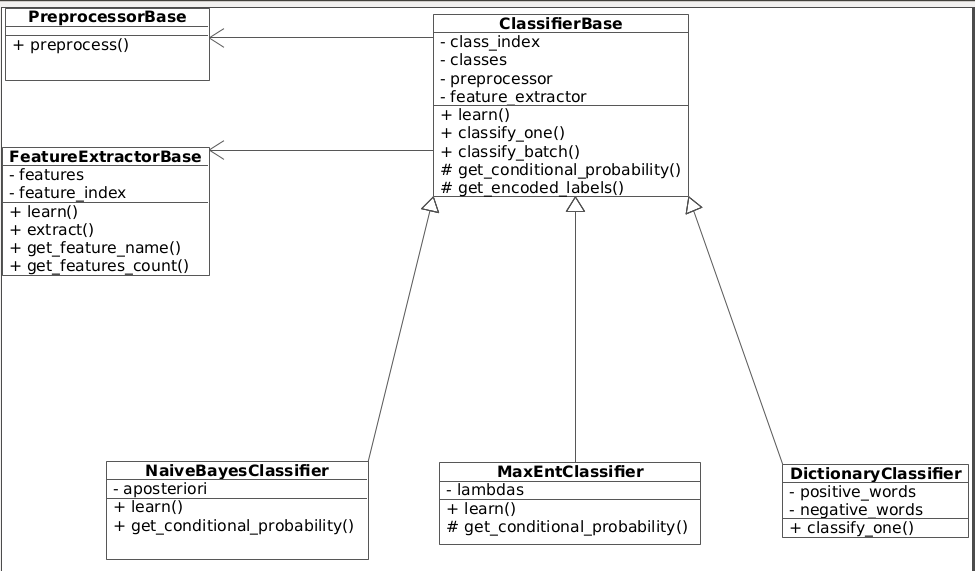
\includegraphics[scale=0.4, trim=1.5mm 2mm 2mm 2.6mm, clip]{../resources/uml/diag1.png}
\caption{Диаграмма классов классификаторов}
\label{gr:classifiers}
\end{center}
\end{figure} 

\begin{figure}[!Ht]
\begin{center}
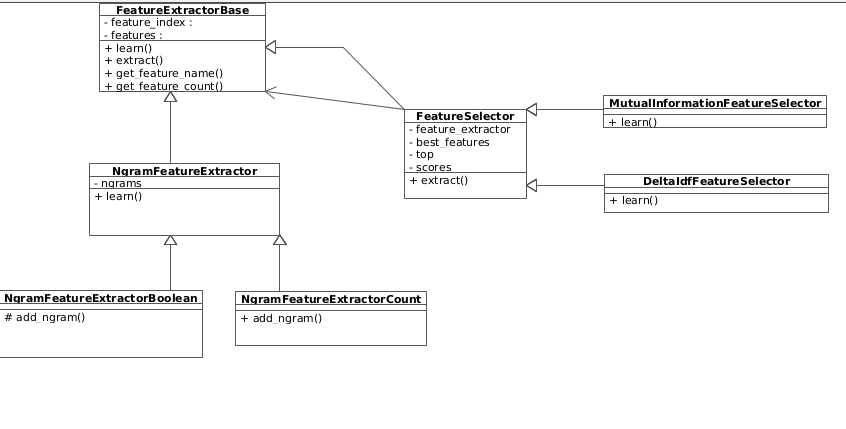
\includegraphics[scale=0.5, trim=0mm 0mm 0mm 1.5mm, clip]{../resources/uml/diag2.png}
\caption{Диаграмма классов для выделителей признаков}
\label{gr:extractors}
\end{center}
\end{figure} 

\begin{figure}[!Ht]
\begin{center}
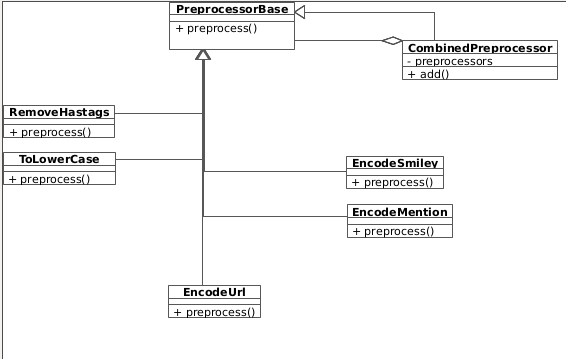
\includegraphics[scale=0.6, trim=1.2mm 10mm 0mm 1mm, clip]{../resources/uml/diag3.png}
\caption{Диаграмма классов для предобработчиков}
\label{gr:preprocessors}
\end{center}
\end{figure} 

\clearpage{}

\subsection{Модуль twitter\_api\_wrapper}
\begin{figure}[!ht]
\begin{center}
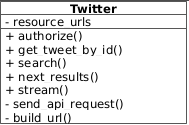
\includegraphics[scale=0.4, trim=0mm 0mm 0mm 0mm, clip]{../resources/uml/diag4.png}
\caption{Диаграмма классов клиента для Twitter}
\label{gr:preprocessors}
\end{center}
\end{figure} 

\subsection{Веб-приложение}
Веб-приложение было разработано при помощи веб-фреймворка Django.
Интерфейс разработан с помощи css-фреймворка ZURB Foundation.

На главной странице пользователь может ввести название
сущности, интересующей его. 
\begin{figure}[!ht]
\begin{center}
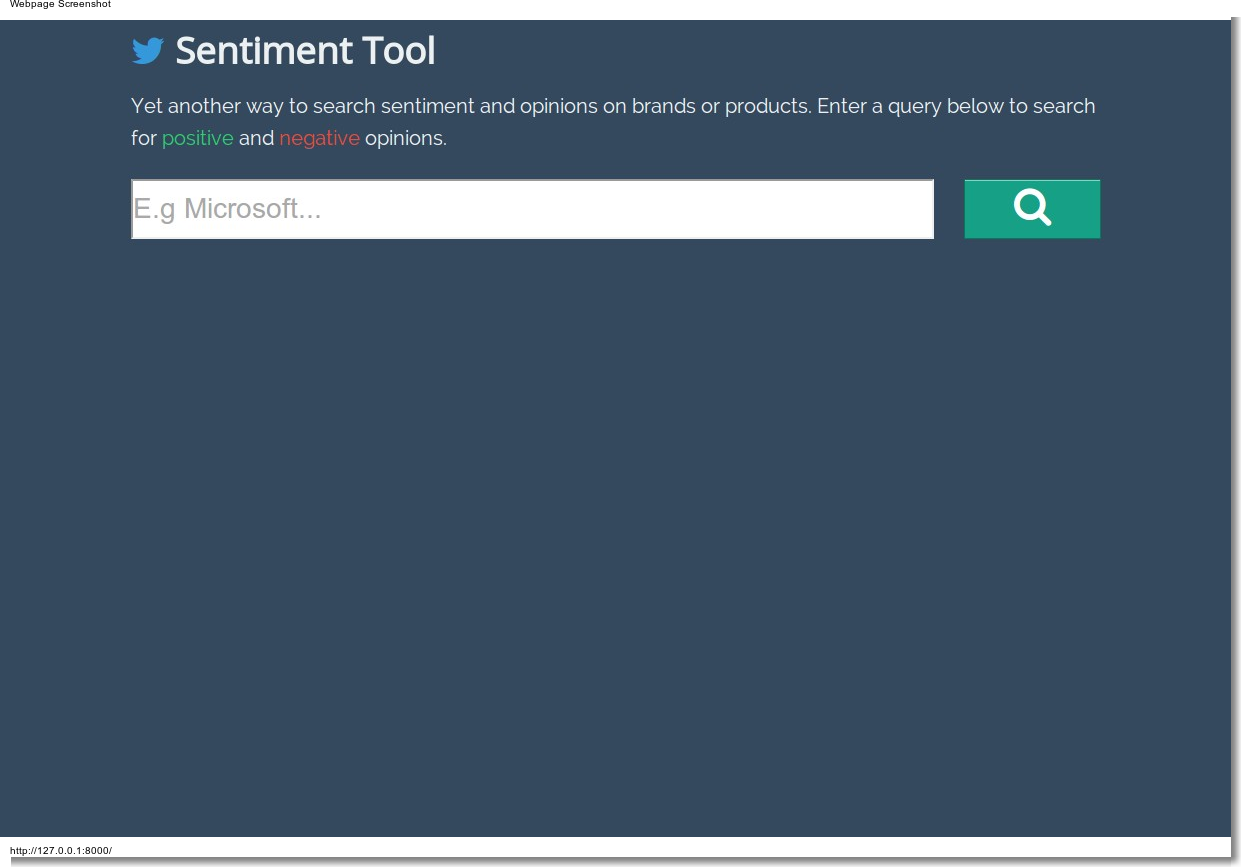
\includegraphics[scale=0.4, trim=20mm 60mm 20mm 10mm, clip]{../resources/screens/main.png}
\caption{Главная страница приложения}
\label{gr:mainpage}
\end{center}
\end{figure} 


После того, как пользователь кликнул на кнопку поиска, происходит ajax-запрос
к серверу. Сервер возвращает уже классифицированные сообщения в 
формате JSON. По умолчанию показываются последние 400 сообщений.

\begin{figure}[!ht]
\begin{center}
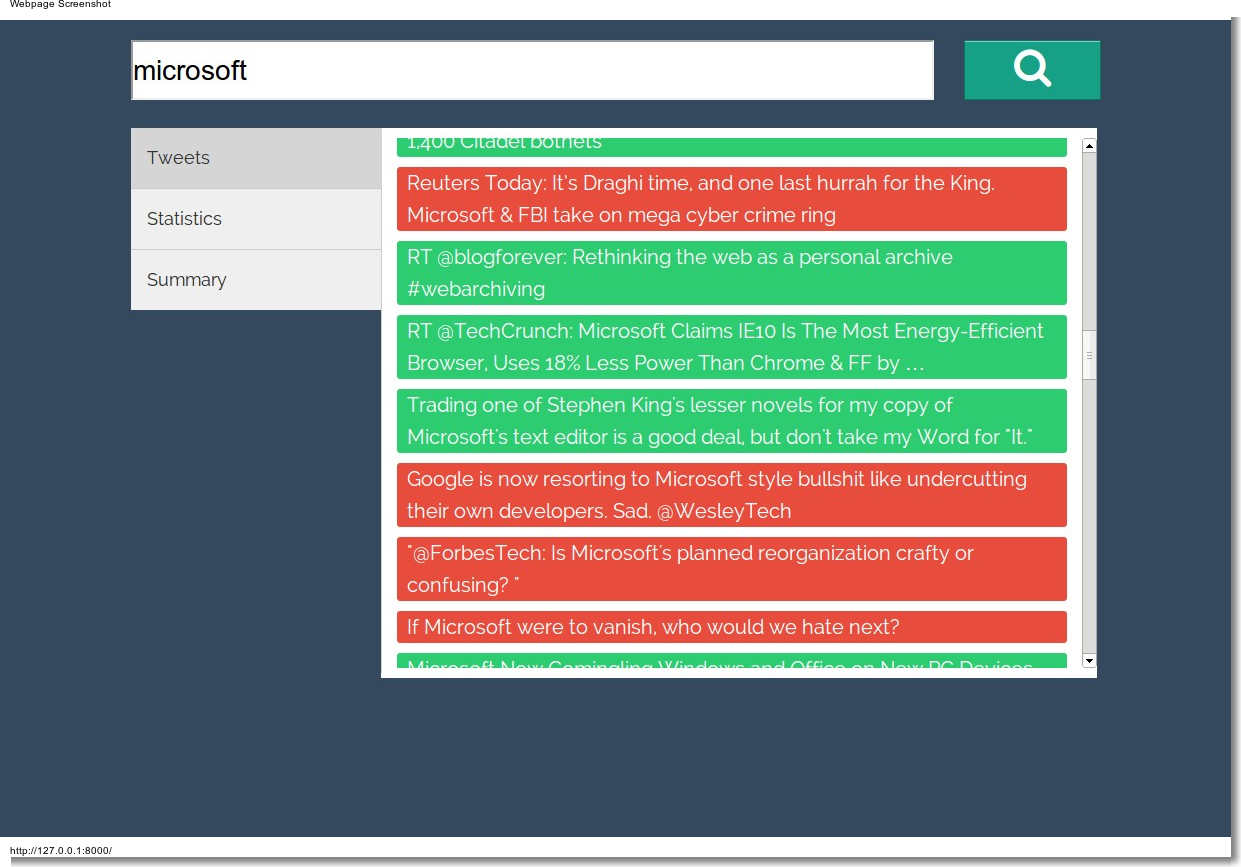
\includegraphics[scale=0.4, trim=20mm 60mm 20mm 10mm, clip]{../resources/screens/tweets.png}
\caption{Вкладка сообщений. Сообщения, имеющие отрицательную тональность подсвечены красным, положительную --- зелёным, нейтральную --- тёмно-синим.}
\label{gr:messages}
\end{center}
\end{figure} 

На вкладке ``Statistics'' (статистика) отображается количество сообщений каждой категории,
а также круговая диаграмма для того, чтобы быстро оценить общее мнение
об объекте поиска.
\begin{figure}[!ht]
\begin{center}
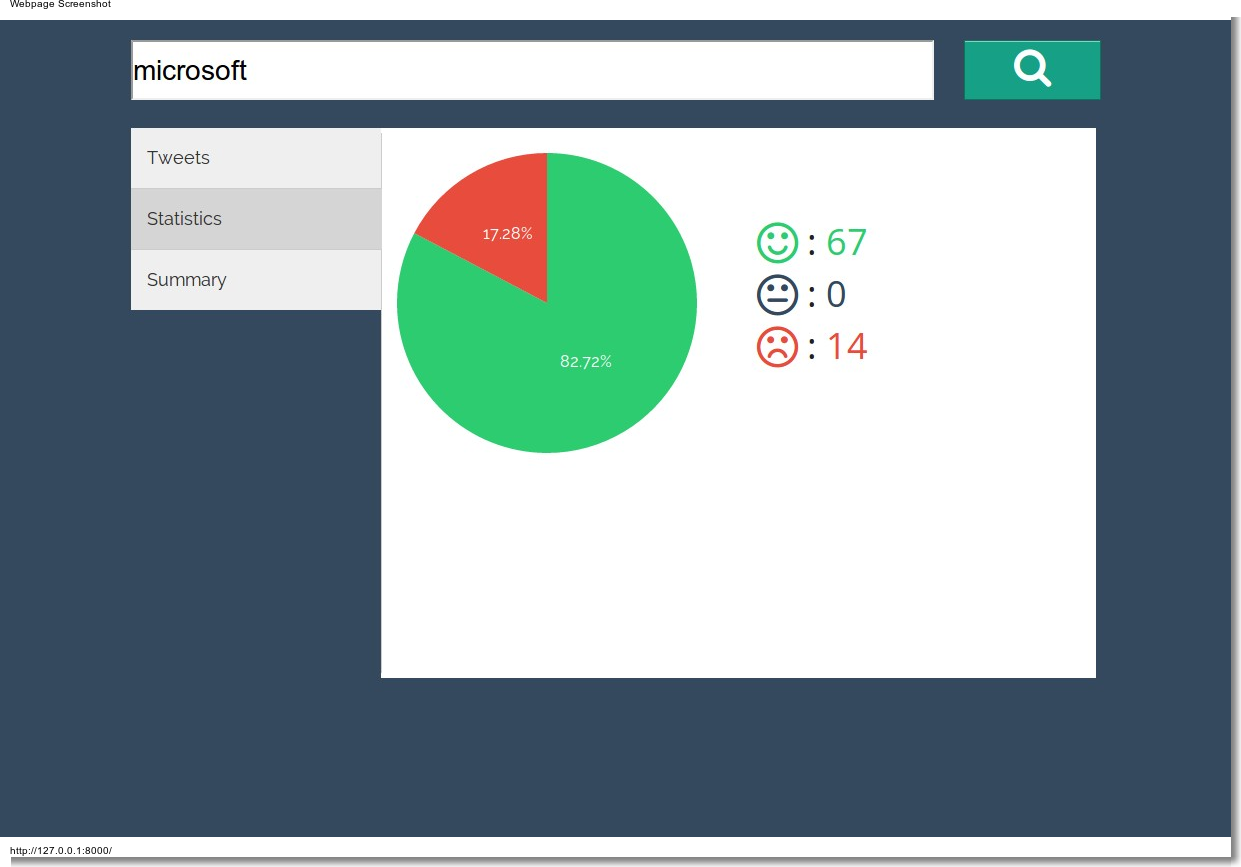
\includegraphics[scale=0.4, trim=20mm 60mm 20mm 10mm, clip]{../resources/screens/statistics.png}
\caption{Вкладка статистики}
\label{gr:stats}
\end{center}
\end{figure} 


На вкладке ``Summary'' (сводка) отображаются два облака слов --- положительное 
(популярные слова, употребляющиеся в позитивном контексте) и отрицательное.
Размер слова пропорционален логарифму частоты употребления.
\begin{figure}[!ht]
\begin{center}
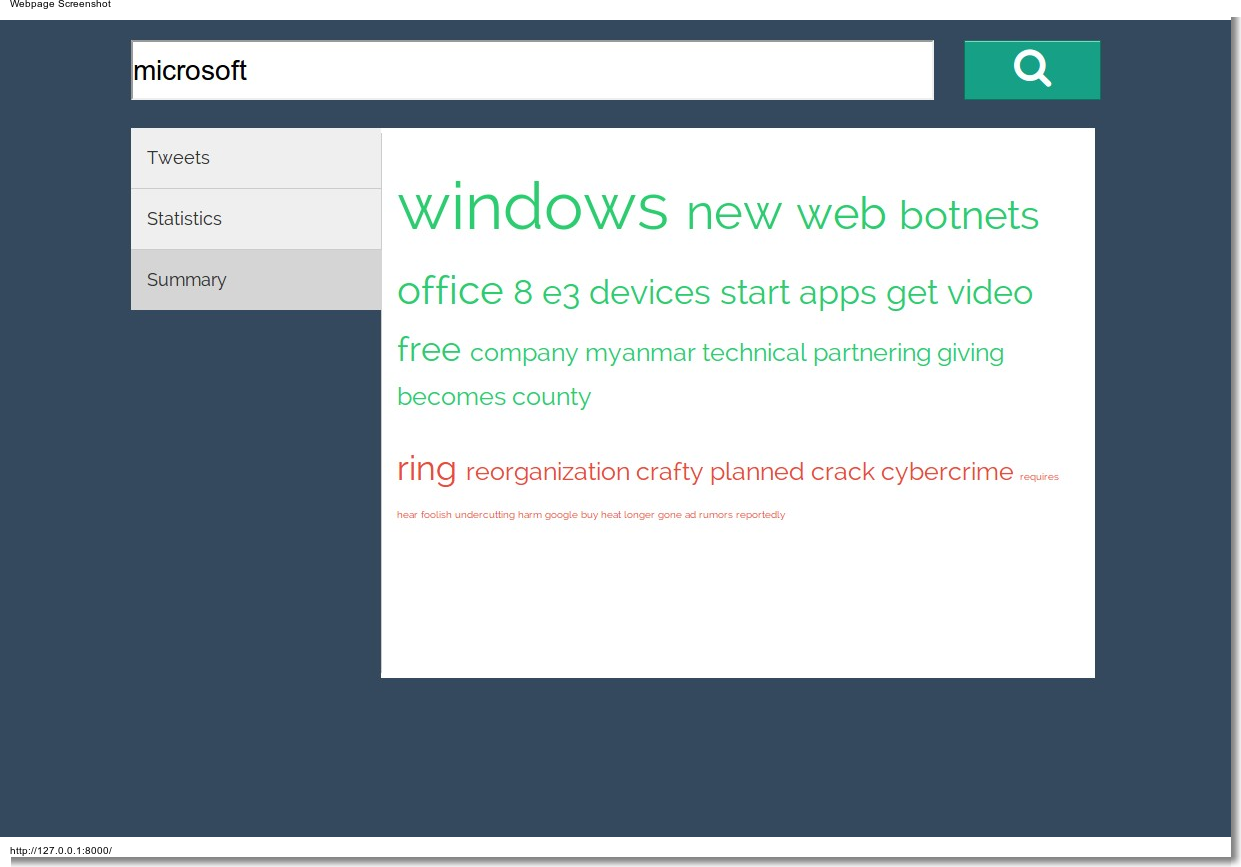
\includegraphics[scale=0.4, trim=20mm 60mm 20mm 10mm, clip]{../resources/screens/summary.png}
\caption{Вкладка сводки}
\label{gr:summary}
\end{center}
\end{figure} 

\clearpage{}
\newpage
\section*{Заключение}
\addcontentsline{toc}{section}{\hspace{7mm}Заключение}
\newpage

\addcontentsline{toc}{section}{\hspace{7mm}Список литературы}
\begin{thebibliography}{0}
\bibitem{wikisent}
Википедия. Анализ тональности текста. --- \\
\href{http://ru.wikipedia.org/wiki/%D0%90%D0%BD%D0%B0%D0%BB%D0%B8%D0%B7_%D1%82%D0%BE%D0%BD%D0%B0%D0%BB%D1%8C%D0%BD%D0%BE%D1%81%D1%82%D0%B8_%D1%82%D0%B5%D0%BA%D1%81%D1%82%D0%B0}{http://ru.wikipedia.org/wiki/анализ\_тональности\_текста}

\bibitem{dimresearch}
The Impact Of Customer Service On Customer Lifetime Value. --- \url{http://www.zendesk.com/resources/customer-service-and-lifetime-customer-value}

\bibitem{aif}
Любителей покупать в интернете не отвадить обманом. --- \url{http://www.aif.ru/mymoney/article/54692}

\bibitem{medianation}
Как отзывы на Яндекс.Маркет влияют на продажи. --- \url{http://www.medianation.ru/blog/kak-otzyvy-na-yandeks-market-vliyayut-na-prodazhi.php}

\bibitem{twitter_users}
Аудитория Twitter выросла на 60 миллионов человек за год. --- \url{http://lenta.ru/news/2013/03/21/twohundred/}

\bibitem{Pang2008}
Pang B., Lee L. Opinion Mining and Sentiment Analysis // Foundations and 
Trends in Information Retrieval, v.2 n.1-2, January, 2008 - pp.1-135.

\bibitem{Go2009}
Go A., Bhayani R., Huang L. Twitter Sentiment Classification using Distant Supervision // Processing , 2009, pp.1-6 .

\bibitem{Liu2010}
Bing Liu. Sentiment Analysis: A Multi-Faceted Problem // IEEE Intelligent Systems, 2010

\bibitem{wiki_middling}
Викисловарь. Посредственный --- \href{http://ru.wiktionary.org/wiki/%D0%BF%D0%BE%D1%81%D1%80%D0%B5%D0%B4%D1%81%D1%82%D0%B2%D0%B5%D0%BD%D0%BD%D1%8B%D0%B9}{http://ru.wiktionary.org/wiki/посредственный}

\bibitem{Liu2010a}
Bing Liu. Sentiment Analysis and Subjectivity // Handbook of Natural Language Processing, 2010

\bibitem{Wiegand2010}
Wiegand M., Balahur A., Roth B., Klakow D., Montoyo. A. A Survey on the Role of Negation in Sentiment Analysis // Workshop on Negation and Speculation in Natural Language Processing, 2010

\bibitem{Tsur2010}
Oren T., Dmitry D., Ari R. ICWSM – A Great Catchy Name: Semi-Supervised Recognition of Sarcastic Sentences in Online Product Reviews // AAAI Conference on Artificial Intelligence, 2010 

\bibitem{Saif2012}
Saif H., He Y., Alani H. Alleviating Data Sparsity for Twitter Sentiment Analysis // Workshop on Making Sense of Microposts, 2012

\bibitem{streaming}
Twitter Streaming API --- \url{https://dev.twitter.com/docs/streaming-apis}

\bibitem{Lin2012}
Lin J., Kolcz A. Large-Scale Machine Learning at Twitter // ACM SIGMOD International Conference on Management of Data, New York, 2012

\bibitem{sentiment_mapreduce}
Basic sentiment analysis using MapReduce --- \url{http://www.alex-hanna.com/tworkshops/lesson-6-basic-sentiment-analysis/}

\bibitem{Irokez2012}
Обучаем компьютер чувствам (sentiment analysis по-русски) --- \url{http://habrahabr.ru/post/149605/}

\bibitem{rule_romip1}
Kan D. Rule-based approach to sentiment analysis // Sentiment Analysis Track at ROMIP, 2011

\bibitem{rule_romip2}
Паничева П. Сиcтема cентиментного анализа ATEX, оcнованная
на правилах, при обработке текcтов различных тематик // Sentiment Analysis Track at ROMIP, 2012

\bibitem{sentiwordnet}
SentiWordNet --- \url{http://sentiwordnet.isti.cnr.it/}

\bibitem{anew}
Affective Norms for English Words (ANEW) --- \url{http://csea.phhp.ufl.edu/media/anewmessage.html}

\bibitem{Manning2008}
Manning D., Raghavan P., Schütze H. Introduction to Information Retrieval // Cambridge University Press, 2008

\bibitem{wiki_vectorspace}
Википедия. Векторная модель --- \href{http://ru.wikipedia.org/wiki/%D0%92%D0%B5%D0%BA%D1%82%D0%BE%D1%80%D0%BD%D0%B0%D1%8F_%D0%BC%D0%BE%D0%B4%D0%B5%D0%BB%D1%8C}{http://ru.wikipedia.org/wiki/Векторная\_модель}

\bibitem{classifier_performance} 
Оценка классификатора (точность, полнота, F-мера) --- \url{http://bazhenov.me/blog/2012/07/21/classification-performance-evaluation.html}

\bibitem{naive_bayes}
Наивный байесовский классификатор --- \url{http://bazhenov.me/blog/2012/06/11/naive-bayes.html}

\bibitem{Pang2002}
Pang B., Lee L., Vaithyanathan S. Thumbs up? Sentiment Classification using Machine Learning Techniques // ACL-02 conference on Empirical methods in natural language processing, 2002, v. 10, pp. 79-86

\bibitem{Sanders}
Twitter Sentiment Corpus --- \url{http://www.sananalytics.com/lab/twitter-sentiment/}

\bibitem{SemEval2013}
SemEval-2013 --- \url{http://www.cs.york.ac.uk/SemEval2013-2013/task2/}

\bibitem{emoticons}
Wikipedia. List of emoticons --- \url{http://en.wikipedia.org/wiki/List_of_emoticons}

\bibitem{dictionary}
Opinion Lexicon --- \url{http://www.cs.uic.edu/~liub/FBS/sentiment-analysis.html#lexicon}

\bibitem{wseas2005}
Ikonomakis M., Kotsiantis S., Tampakas V. Text Classification Using Machine Learning Techniques // WSEAS TRANSACTIONS on COMPUTERS, Iss. 8, Vol. 4, 2005, pp. 966-974

\bibitem{mutualinformation}
Взаимная информация --- \url{http://bazhenov.me/blog/2012/12/10/feature-selection.html}
\end{thebibliography}

\end{document}
